\selectlanguage{spanish}
\let\textcircled=\pgftextcircled
\chapter {Marco Teórico}
\label{chap:teorico}

\initial{A} continuación se introducen los conceptos y características de los modelos de Markov, seguido de la especialización en modelos ocultos, utilizados para modelar una red de tráfico. Finalmente, se presenta el algoritmo de Viterbi, fundamental para el método de estimación desarrollado. Los temas abordados son acompañados por ejemplos concretos que explican la aplicación de los modelos descritos. 

\section{Cadenas de Markov}

\subsection{Reseña}
Un proceso o sucesión de eventos que se desarrolla en el tiempo en el cual el resultado en cualquier etapa contiene algún elemento que depende del azar se denomina proceso aleatorio o proceso estocástico. Por ejemplo, la sucesión podría ser las condiciones del tiempo en Paraná en una serie de días consecutivos: el tiempo cambia día a día de una manera que en apariencia es algo aleatoria. O bien, la sucesión podría consistir en los precios de las acciones que cotizan en la bolsa en donde otra vez interviene cierto grado de aleatoriedad.
Un ejemplo simple de un proceso estocástico es una sucesión de ensayos de Bernoulli, por ejemplo, una sucesión de lanzamientos de una moneda. En este caso, el resultado en cualquier etapa es independiente de todos los resultados previos (esta condición de independencia es parte de la definición de los ensayos de Bernoulli). Sin embargo, en la mayoría de los procesos estocásticos, cada resultado depende de lo que sucedió en etapas anteriores del proceso. Por ejemplo, el tiempo en un día determinado no es aleatorio por completo sino que es afectado en cierto grado por el tiempo de días previos. El precio de una acción al cierre de cualquier día depende en cierta medida del comportamiento de la bolsa en días previos.
El caso más simple de un proceso estocástico en que los resultados dependen de otros, ocurre cuando el resultado en cada etapa sólo depende del resultado de la etapa anterior y no de cualquiera de los resultados previos. Tal proceso se denomina proceso de Markov o cadena de Markov (una cadena de eventos, cada evento ligado al precedente). Estas cadenas reciben su nombre del matemático ruso Andrei Andreevitch Markov (1856-1922). Como mencionamos antes, estas cadenas tienen memoria, recuerdan el último evento y eso condiciona las posibilidades de los eventos futuros. Esto justamente las distingue de una serie de eventos independientes como el hecho de tirar una moneda. Este tipo de proceso presenta una forma de dependencia simple, pero muy útil en muchos modelos, entre las variables aleatorias que forman un proceso estocástico. Se utilizan, por ejemplo, en frameworks para diseñar y resolver problemas de decisión \cite{beccuti2007framework}, para la medición de fiabilidad y rendimiento de sistemas de software \cite{goel1899markovian}, entre otros.

\subsection{Definición}
Una cadena de Markov es una sucesión de ensayos similares u observaciones en la cual cada ensayo tiene el mismo número finito de resultados posibles y en donde la probabilidad de cada resultado para un ensayo dado depende sólo del resultado del ensayo inmediatamente precedente y no de cualquier resultado previo.

\subsection{Propiedad de Markov}

Dada una secuencia de variables aleatorias $X_1, X_2, X_3, ... , X_n$

\begin{figure}[htp]
\centering
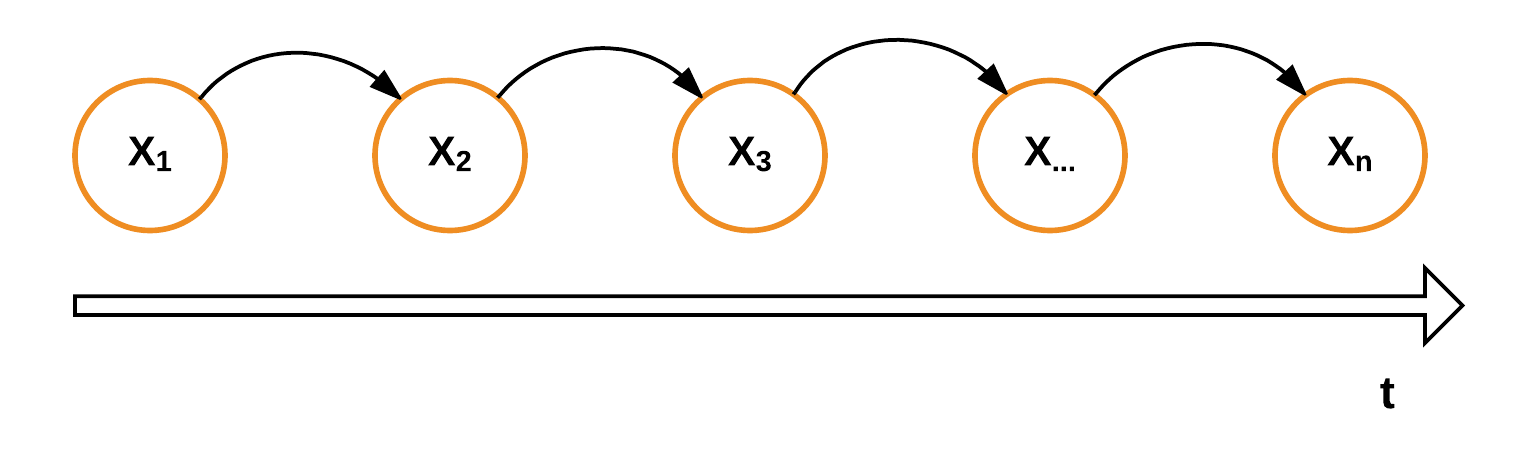
\includegraphics[scale=0.8]{images/va.png}
\caption{Secuencia de variables aleatorias}
\end{figure}

tales que el valor de $X_n$ es el estado del proceso en el tiempo $n$. Si la distribución de probabilidad condicional de $X_{n+1}$ en estados pasados es una función de $X_n$ por sí sola, entonces:
\begin{align*}
P(X_{n+1}=x_{n+1}|X_n=x_n, X_{n-1}=x_{n-1}, ... ,X_2=x_2, X_1=x_1)=P(N_{n+1}=x_{n+1}|X_n=x_n)     
\end{align*}

Donde $x_i$ es el estado del proceso en el instante $t=i$. Esta identidad es la denominada propiedad de Markov: El estado en $t=i+1$ sólo depende del estado en $t=i$ y no de la evolución anterior del sistema.

Si un estado depende de otro además del inmediatamente anterior, este es un proceso de Markov de un orden mayor a uno. Por ejemplo, un proceso de segundo orden describe un proceso en el cual el estado depende de los dos estados anteriores.
Los procesos de Markov también se les llama Cadenas de Markov.

\textbf{Matriz de Transición}

Consideremos un proceso de Markov en que el sistema posee N estados posibles, dados por los números $1, 2, 3, ... , \mathrm{N}$. Denotemos $a_{ij}$ a la probabilidad de que el sistema pase al estado $j$ después de cualquier ensayo en donde su estado era $i$ antes del ensayo. Los números $a_{ij}$ se denominan probabilidades de transición y la matriz $A={a_{ij}}$ (N$\times$N)  se conoce como matriz de transición del sistema.


\textbf{Observaciones sobre la Matriz de Transición}
\begin{enumerate}
\item La suma $a_{i1}+a_{i2}+...+a_{i\mathrm{N}}=1$. Esta suma representa la probabilidad de que el sistema pase a uno de los estados $1, 2, ... , \mathrm{N}$ dado que empieza en el estado $i$. Ya que el sistema ha de estar en uno de estos N estados, la suma de probabilidades debe ser igual a 1. Esto significa que los elementos en cualquier columna de la matriz de transición deben sumar 1.
\item Cada elemento $a_{ij} \geq 0$
\end{enumerate}


\textbf{Representación gráfica}
\begin{figure}[htp]
\centering
\captionsetup{width=.7\linewidth}
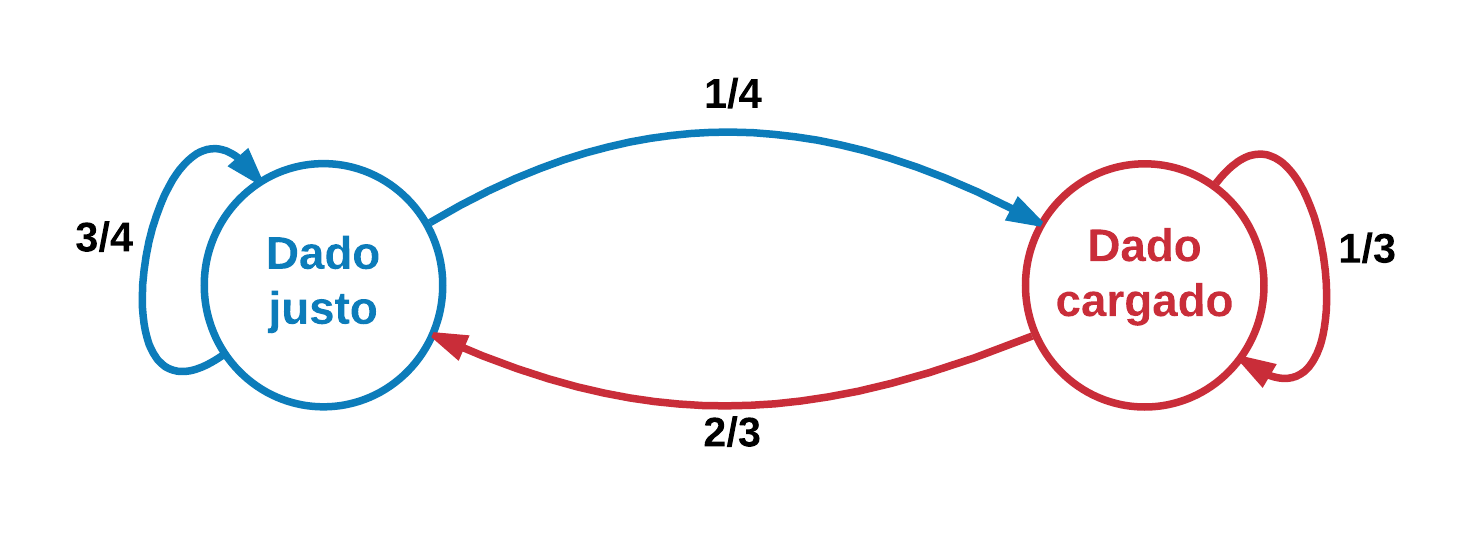
\includegraphics[width=.7\linewidth]{images/representacion_markovsimple.png}
\caption{Representación gráfica de un sistema de dos estados: dado justo y dado cargado}
\label{fig:markovsimple}
\end{figure}

A modo de ejemplo, consideremos el siguiente caso: Un casino deshonesto tiene dos dados, uno justo y otro cargado. El casino alterna entre los dados con cierta frecuencia. En la Figura \ref{fig:markovsimple} se observa un gráfico de la representación en un grafo de las transiciones con sus respectivos valores de probabilidad. Los círculos se corresponden con estados y los arcos, los cuales poseen dirección, son las direcciones de posibles transiciones. Cabe destacar también que debe cumplir con las observaciones mencionadas anteriormente.


\subsection{Aplicación}

Las cadenas de Markov proporcionan un sistema muy útil para crear e implementar un proceso de toma de decisiones que permita evaluar posibles escenarios y se utiliza para predecir con mayor exactitud comportamientos futuros. Estas tienen muchas aplicaciones en el mundo real, destacando su uso en negocios, política, finanzas, deportes, salud, genética, física, economía y un largo etcétera.
Algunos ejemplos puntuales de aplicaciones son algoritmos de posicionamiento web\cite{backaaker2012google} (en este caso la cadena de Markov puede ser utilizada para hacer predicciones futuras de navegación para los usuarios individuales); modelos financieros para optimización de acciones\cite{yang2011research}; análisis de juegos como el béisbol; señal y procesamiento de imágenes\cite{bishop2007pattern}; reconocimiento de imágenes\cite{bishop2007pattern}; reconocimientos de patrones \cite{bishop2007pattern}; seguros de vida y diversas aplicaciones en marketing\cite{datong2011markov}.

\section{Modelos Ocultos de Markov}

\subsection{Reseña}
Un modelo oculto de Markov (o HMM por sus siglas en inglés) es la representación de un proceso estocástico que consta de dos mecanismos interrelacionados: una cadena de Markov de primer orden subyacente, con un número finito de estados, y un conjunto de funciones aleatorias, cada una de las cuales está asociada a un estado. En un instante discreto de tiempo se supone que el proceso está en un estado determinado y que genera una observación mediante la función aleatoria asociada. Al instante siguiente, la cadena subyacente de Markov cambia de estado siguiendo su matriz de probabilidades de transición entre estados, produciendo una nueva observación mediante la función aleatoria correspondiente. El observador externo sólo ``ve'' la salida de las funciones aleatorias asociadas a cada estado, siendo incapaz de observar directamente la secuencia de estados de la cadena de Markov. De ahí el nombre de modelo oculto.

\subsection{Definición}
Un modelo oculto de Markov queda, entonces, caracterizado por los siguientes elementos:
\begin{enumerate}
\item El conjunto finito de N estados de la cadena de Markov de primer orden.
Aunque los estados están ocultos, en muchas aplicaciones prácticas éstos tienen un significado físico que es preciso considerar. Se denotará como $S=\{S_i\}$ $i=1...\mathrm{N}$ a este conjunto de estados y al estado en el tiempo $t$ como $q_t$.
\item El conjunto de probabilidades de transición entre estados. Denotando los instantes de tiempo regularmente espaciados asociados a los cambios de estados como $t=1,2,...,\mathrm{T}$. Una descripción probabilística completa de una cadena requeriría, en general, especificaciones sobre el estado actual en el instante $t$ y de todos los estados predecesores. Para el caso especial de una cadena de Markov de primer orden, esta descripción probabilística se trunca en el estado actual y el último predecesor, es decir,
\begin{align*}
P(q_t=S_j | q_{t-1}=S_i, q_{t-2}=S_k, ...)=P(q_t=S_j | q_{t-1}=S_i)    
\end{align*}
\end{enumerate}

Además, se considera que esta última probabilidad es independiente del tiempo (propiedad de homogeneidad temporal), lo cual da lugar a un conjunto de probabilidades de transición entre estados que se denotará con una matriz $A = \{ a_{ij} \}$ i,j = 1 ... N, donde
\begin{align*}
a_{ij}=P(q_t=S_j | q_{t-1}= S_i)        & & \text{i, j = 1, ... ,N}
\end{align*}


Este conjunto de probabilidades determinará la topología del modelo. Así, para un modelo en que cada estado puede ser alcanzado desde cualquier otro en un sólo paso, $a_{i,j}>0$  i, j=1, ... , N. En general, los modelos pueden tener $a_{ij}=0$ para una o más parejas de valores (i,j). En cualquier caso deben verificar

\begin{align}
\sum_{j=1}^{N} a_{ij}=1        & &\text{i=1, ... , N}    \\
a_{ij}\geq0                    & &\text{i,j=1, ... , N}
\end{align}

3) La distribución de probabilidad de estados iniciales, que se denotará como $\{\pi_i\}$ i=1,...,N, definida de la forma
\begin{align}
\pi_i=P(q_1=S_i)               & &\text{i=1, ... , N}
\end{align}
Siendo $q_1$ el estado en $t=1$ \\
Como tales probabilidades, también deben verificar
\begin{align}
\sum_{i=1}^{\mathrm{N}} \pi_i=1          & &\text{i=1, ... , N} \\
\pi_i \geq 0                             & &\text{i=1, ... , N}
\end{align}


4) Las probabilidades de generación de observaciones, que caracterizan el proceso asociado a cada uno de los estados del modelo y que se denotará como $\mathrm{B}=\{b_j(\mathrm{O}_t)\}$ j=1, ... , N, con
\begin{align}
b_j(\mathrm{O}_t)=P(\mathrm{O}_t | q_t=S_j)          & &\text{j=1, ... , N}
\end{align}

en donde O$_t$ representa el valor de la observación en el instante $t$, correspondiente a la secuencia de observaciones O=$\{\mathrm{O}_t\}$     t=i, ... , T. Se supone que el proceso de generación de observaciones es independiente del tiempo y que únicamente depende del estado actual del modelo. Hay que hacer notar que en algunas variantes de modelos ocultos de Markov estas probabilidades de observación están asociadas a las transiciones, en lugar de a los estados.

\begin{figure}[!htp]
\centering
\captionsetup{width=.6\linewidth}
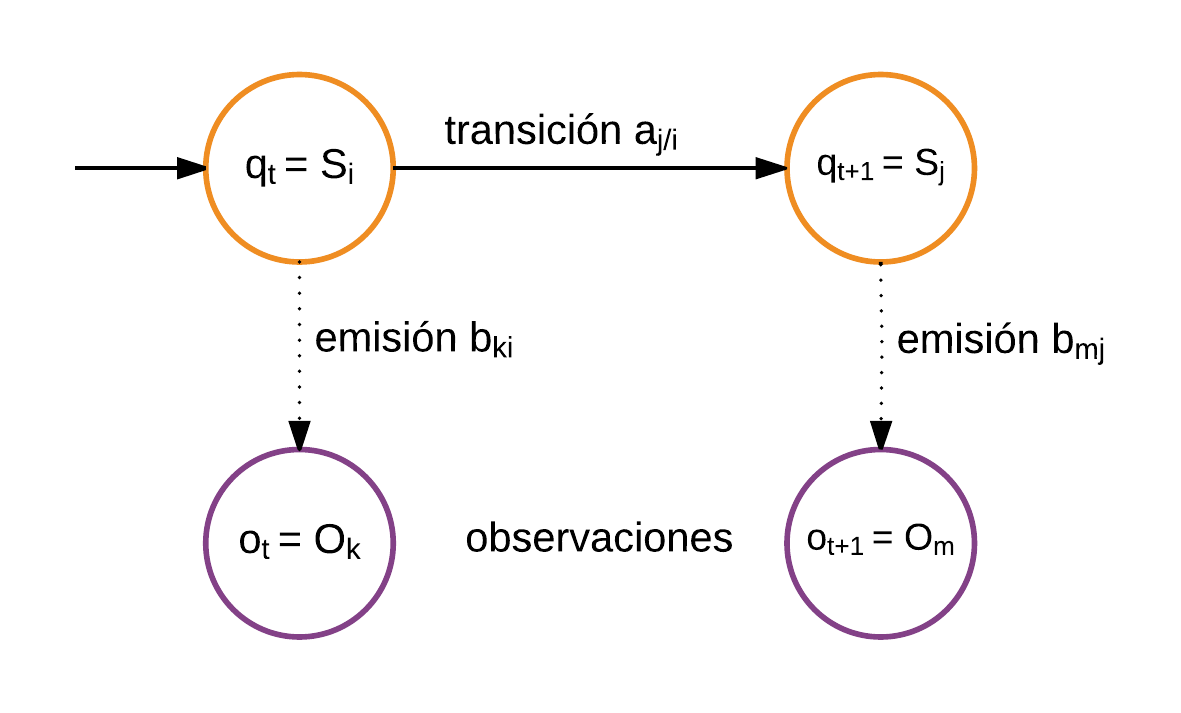
\includegraphics[width=.6\linewidth]{images/emision_hmm.png}
\caption{Secuencia de variables aleatorias con emisión de símbolos $o_t=\mathrm{O}_k$}
\label{fig:emisioneshmm}
\end{figure}

De esta forma el modelo HMM queda definido por la especificación de los conjuntos $\pi$, A y B, que implícitamente fijan el valor de N. Por ello, se suele utilizar la notación compacta
\begin{align*}
\lambda = (\pi,\mathrm{A},\mathrm{B})    
\end{align*}

para referirse a un determinado modelo $\lambda$.

Una representación esquemática de un modelo oculto de Markov de dos estados ergódicos (con ningún elemento de la matriz de transiciones nulo) es el caso del casino deshonesto (Figura \ref{fig:hmmejemplo}). Aquí, los estados “dado justo” y “dado cargado”, se corresponden a los valores que puede tomar la variable oculta $q_t$ (no observables directamente) en el instante de tiempo t. $\mathrm{O}_t$ es el valor de un dado arrojado en el mismo instante t. En este caso, los valores 1-6 forman el conjunto de posibles valores observables (6 símbolos posibles). A modo de ejemplo, se expresan las probabilidades de arrojar cada valor según el dado, o bien, $P(\mathrm{O}_t|q_t=S_j)$, j = \{dadojusto, dadocargado\}, equiprobables para el dado justo y mayor probabilidad para el valor “6”, en el dado cargado. De la Figura \ref{fig:hmmejemplo} queda claro que el valor de la variable observada sólo depende del valor de la variable oculta (ambas en el instante t).

%Llegue hasta aca 28/4
\begin{figure}[!htp]
\centering
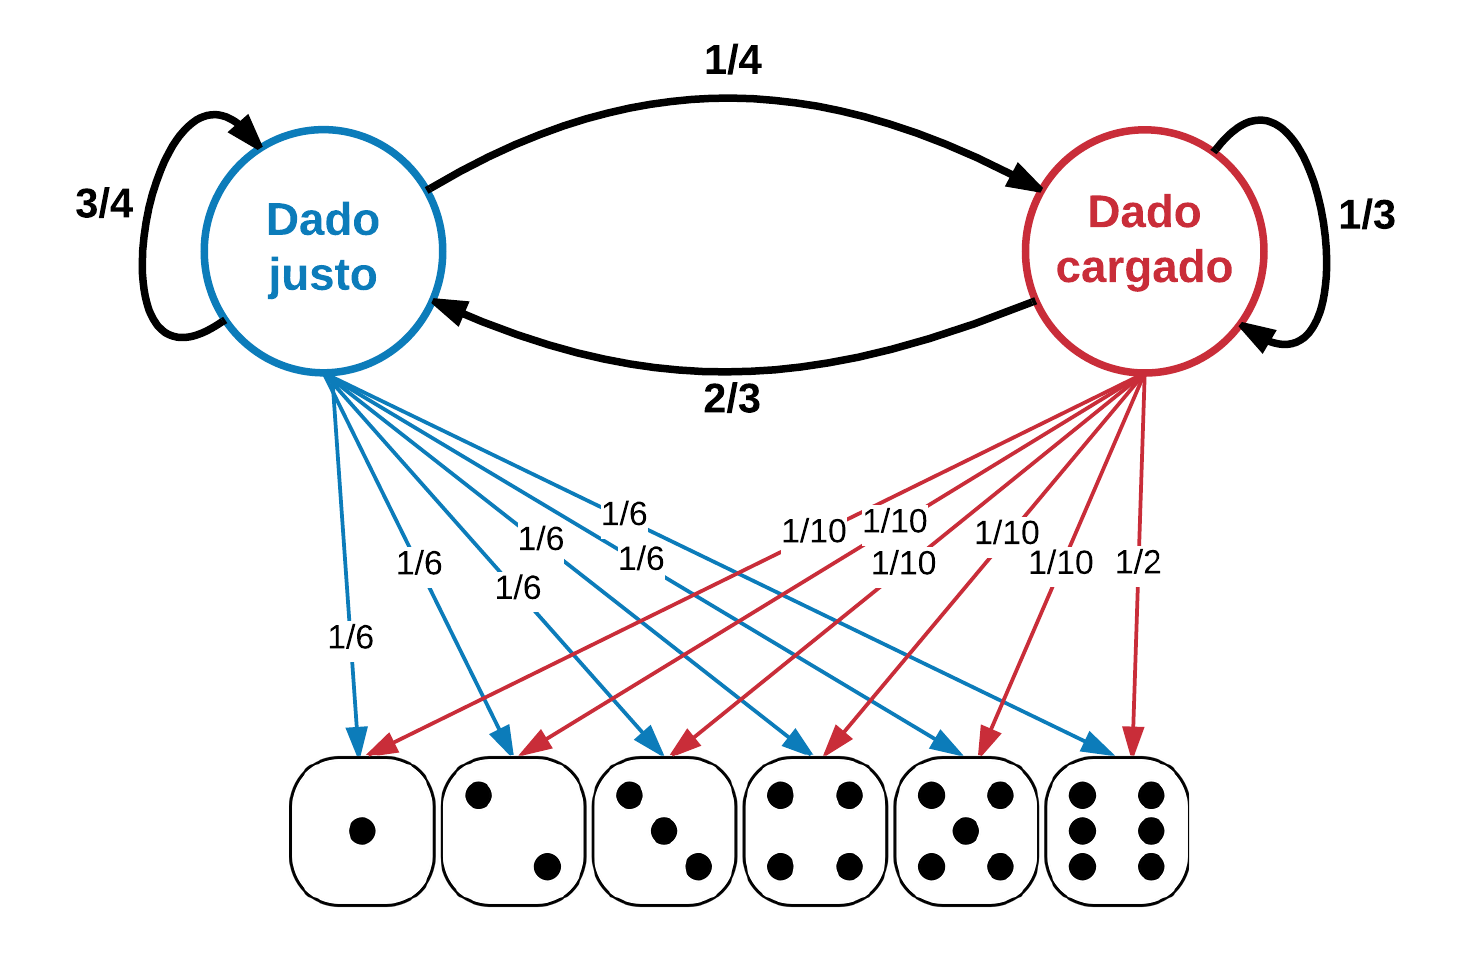
\includegraphics[scale=0.2]{images/hmm_ejemplo.png}
\caption{Modelo Oculto de Markov del casino deshonesto}
\label{fig:hmmejemplo}
\end{figure}


La naturaleza de las probabilidades de generación de observaciones de cada estado $b_j(\mathrm{O}_t)$ es la diferencia fundamental entre los distintos tipos de modelos. En los llamados modelos discretos (DHMM), estas probabilidades están representadas a través de distribuciones de probabilidad discretas, ya que las observaciones $\mathrm{O}_t$ toman valores dentro de un conjunto discreto y finito de símbolos llamado alfabeto V={v$_k$}   k=1, ... , M, siendo M el tamaño del alfabeto. Las probabilidades de observación forman, pues, un conjunto que se denota como una matriz $\mathrm{B}=\{b_j(k)\}$  j=1, ... , N; k=1, ... , M, donde
\begin{align}
b_j(k)=P(v_k\text{ en }t | q_t=S_j)     & & \text{j = 1,... , N }   & \text{ k=1,... , M}
\end{align}

Por ser probabilidades estos parámetros deben verificar
\begin{align}
\sum_{j=1}^{N} b_j(k)=1                 & &  \text{k=1, ... , M} \\
b_j(k) \geq 0      & & \text{k=1, ... , M} &  \text{ j=1, ... , N}
\end{align}

En los modelos continuos (CHMM), las probabilidades de observación están representadas a través de funciones de densidad de probabilidad multivariadas, ya que las observaciones toman valores dentro de un espacio continuo multidimensional. 

\subsection{Problemas en HMM} \label{ssec:problemashmm}

Una vez definido el modelo para un determinado proceso, surgen tres problemas básicos de interés que deben resolverse de cara a posibles aplicaciones prácticas:
\begin{description}
\item [Problema de evaluación] Dada una secuencia de observaciones $\mathrm{O}=\{\mathrm{O}_t\}$ t=1, ... , T y un modelo $\lambda=(\pi, A, B)$, cómo evaluar eficientemente $P(O |\lambda )$, la probabilidad de la secuencia de observación dado el modelo. Esta probabilidad se puede utilizar para clasificar las secuencias de observación.
\item [Problema de entrenamiento] Dada una secuencia de observaciones $\mathrm{O}=\{\mathrm{O}_t\}$ t=1, ... , T cómo ajustar los parámetros del modelo $\lambda=(\pi, A, B)$ de forma que se maximice $P(O | \lambda)$, la probabilidad de generación de dicha secuencia por el modelo. Su solución permite desarrollar un método para obtener los parámetros de un modelo en base a secuencias de observaciones que se pretenden modelar.
\item [Problema de decodificación] Dada una secuencia de observaciones $\mathrm{O}=\{\mathrm{O}_t\}$ t=1, ... , T y un modelo $\lambda=(\pi, A, B)$, cómo elegir la correspondiente secuencia de estados $Q=\{q_t\}$ t=1, ... , T que es óptima en algún sentido, que mejor \enquote{explica} las observaciones. Su solución permite obtener información sobre el proceso oculto, por ejemplo, el significado de los estados del modelo. 
\end{description}

\subsection{Aplicación}
El concepto de HMM fue aplicado inicialmente en el campo del reconocimiento automático del habla\cite{rabiner1989tutorial}, donde actualmente es una herramienta casi imprescindible, que ha encontrado aplicación en diversas disciplinas, como el análisis de imágenes\cite{aas1999applications} o la psicología \cite{visser2002fitting}, destacando su uso creciente en bioinformática, donde los HMM están ya bien establecidos\cite{visser2002fitting,baldi2001bioinformatics}, y en el análisis de electroencefalogramas y otras bioseñales\cite{novak2004speech,penny1998gaussian}. Como el área de aplicación es inmensa solo describiremos unos pocos usos con la finalidad de tener una visión clara del futuro de los HMM.

                                                                                                                                                                                                                                                                                                                                                        En lo que respecta a la bioinformática y su relación con los modelos ocultos de Markov, la utilización de los mismos como modelos de perfil fue introducida por Krogh et al. a mediados de los ’90 \cite{eddy1998profile}                                                                                                                                                                                                                                                                                                           . Algunos ejemplos del uso de HMM en el campo de la biología son el descubrimiento de genes, el mapeo de ligamientos genéticos y la predicción de estructura secundaria.
La idea de usar perfiles HMM para la búsqueda en bases de datos es comparar una secuencia con un modelo estadístico que describe una familia o patrón de secuencias al contrario de la simple comparación de partes individuales de dos secuencias. Además, comparando una secuencia con un modelo estadístico se puede obtener información extra.

Por otro lado, en lo que respecta al reconocimiento de voz mediante los modelos ocultos de Markov se sabe que debido a la inercia inherente a los órganos articulatorios, es posible suponer que las características de la señal no varían demasiado en un intervalo corto de tiempo, por lo que es posible realizar un análisis espectral sobre segmentos de señal de esta duración temporal. En los sistemas de reconocimiento de voz mediante técnicas de comparación de patrones se aborda el proceso de reconocimiento sin realizar un modelado de la evolución temporal de esta secuencia de espectros. Los patrones de referencia y de test consisten simplemente en secuencias de espectros y el proceso de comparación se limita a calcular la distancia acumulada entre dichos patrones a lo largo del camino óptimo dado por un algoritmo. En los sistemas basados en modelos ocultos de Markov, se modela la evolución temporal de la secuencia de espectros obtenida de la señal de voz mediante un HMM con el fin de contemplar las diversas fuentes de variabilidad de la señal. Este modelado consiste en la asociación de los estados del HMM a los diferentes tramos de la señal, de forma que las probabilidades de generación de observaciones modelan la variabilidad estadística de las características espectrales de cada tramo, mientras que las probabilidades de transición modelan su secuenciamiento y duración.


\section{Algoritmo de Viterbi}

El problema de decodificación, el cual se basa en un modelo de Markov y una secuencia de observaciones, sobre las cuales debe determinar cuál es la secuencia de estados que mejor la explica, puede ser resuelto calculando todas las combinaciones posibles $Q=\{q_t\}$   t=1, ... , T, eligiendo la de máxima probabilidad. Se calcula, para cada combinación $Q$:
\begin{align}
P(Q,O |\lambda)=\pi_q1b_q1(\mathrm{O}_1)a_{q_1q_2}b_{q_2}(\mathrm{O}_2) ... a_{q_{T-1}q_T}b_{q_T}(\mathrm{O}_T)
\end{align}
Donde $\pi$ es un vector que denota el estado inicial que se considera, O$_t$ las observaciones en los tiempos dados y $b_{q_t}(\mathrm{O}_t)$ que es el valor de la probabilidad de observar O${_t}$ cuando se está en el estado $q$ en el tiempo $t$. En el caso de ejemplo (el casino deshonesto), la observación con la que contamos, o bien, los estados \enquote{observables}, es la secuencia de valores de los dados arrojados. Lo que podremos estimar es, qué partes de la secuencia fueron generadas por un dado justo y qué partes con el dado cargado. Esto mismo podremos verlo en mayor detalle más adelante, junto al ejemplo aplicado.

Existen métodos más eficientes basados en recursión como el algoritmo de Viterbi. Este mismo permite encontrar las secuencias de estados más probables en un modelo oculto de Markov a partir de una observación, es decir, obtiene la secuencia óptima que mejor \enquote{explica} la secuencia de observaciones. Cabe mencionar que el algoritmo de Viterbi es de programación dinámica, si esto no fuera así y fuera iterativo la complejidad sería demasiado grande.

\subsection{Reseña}
Para encontrar la secuencia de estados $Q={q_t}$   t=1, ... , T dada una secuencia de observaciones $\mathrm{O}=\{\mathrm{O}_t\}$     t=1, ... , T se define la variable
\begin{align}
\delta_t(i)=max_{q_1,q_2,...,q_t}\{P(q_1q_2 ... q_t=i, \mathrm{O}_1\mathrm{O}_2 ... \mathrm{O}_t |\lambda )\} 
\end{align}

Considerando lo expuesto anteriormente, en primer lugar definimos la probabilidad parcial $\delta$, que es la probabilidad de alcanzar un estado intermedio particular. Para cada estado intermedio y terminal, hay un camino más probable a ese estado. Llamaremos a estos caminos los \enquote{mejores caminos parciales}. Cada uno de estos mejores caminos parciales tiene una probabilidad asociada, la probabilidad parcial o $\delta$. Entonces, $\delta(i, t)$ es la probabilidad máxima entre todas las secuencias que terminan en el estado i en el tiempo t, y el mejor camino parcial es la secuencia que alcanza esta probabilidad máxima. Tal probabilidad (y camino parcial) existen para cada estado i y tiempo t.\\
Por inducción, se define:
\begin{align}
\delta_{t+1}(j)=max_i\{\delta_t(i)a{ij}\}b_j(\mathrm{O}_{t+1})
\label{eqn:recursionviterbi}
\end{align}


Para recuperar la secuencia de estados de probabilidad máxima es necesario almacenar los valores del argumento que maximizan la ecuación anterior, para cada t y j. Para ello se utiliza la matriz $\psi_t(j)$. En la misma se van almacenando los valores calculados con la ecuación \ref{eqn:recursionviterbi}, para que luego de finalizar con todos los cálculos poder determinar cuál es la secuencia óptima de estados que mejor explique las observaciones dados los valores almacenados en la matriz.


\subsection{Algoritmo}
El algoritmo de Viterbi cuenta con los pasos descritos en el algoritmo (\ref{alg:viterbi}).

\begin{algorithm}
\caption{Algoritmo de Viterbi}\label{alg:viterbi}
\begin{algorithmic}[1]
\Procedure{Viterbi}{}
\BState \emph{1) Inicialización}:
\State $\delta_1(i) \gets \pi_ib_i(\mathrm{O}_1)$ \Comment{i = 1,...,N}
\State $\psi_1(i) \gets 0$
\BState \emph{2) Recursión}:
\State $\delta_t(j) \gets max_{i=1,...,\mathrm{N}} \{ \delta_{t-1}(i)a_{ij}\}b_j(\mathrm{O}_t)$ \Comment{t = 2,...,T  y j=1,...,N}
\State $\psi_t(j) \gets argmax_{i=1,...,\mathrm{N}}\{\delta_{t-1}(i)a_{ij}\} $ \Comment{t = 2,...,T  y j=1,...,N}
\BState \emph{3) Terminación}:
\State $P^*=max_{i=1,...,\mathrm{N}}\{\delta_\mathrm{T}(i)\}$
\State $q_T^*=argmax_{i=1,...,\mathrm{N}}\{\delta_\mathrm{T}(i)\}$
\BState \emph{4) Recursión para obtener la secuencia de estados}:
\State $q_t^*=\psi_{t+1}(q_{t+1}^*)$ \Comment{t = T-1, T-2,...,1}
\EndProcedure
\end{algorithmic}
\end{algorithm}

Hay que destacar que en este caso no se consideran todas las transiciones hasta cada estado, sino solamente aquellas que dan lugar a una probabilidad máxima.

El algoritmo de Viterbi no se utiliza tan sólo para determinar la secuencia de estados óptima, sino también para determinar la probabilidad de una secuencia de observaciones por el camino óptimo.

\subsection{Ejemplo: El casino deshonesto}
A partir del modelo del casino deshonesto y una secuencia de dados arrojados como la siguiente, veremos cómo hallar la secuencia de estados de máxima probabilidad:

3 6 4 

Consideraremos $\pi = \{\frac{1}{2}, \frac{1}{2}\}$ como vector de probabilidades iniciales. La siguiente tabla resume los cálculos de cada secuencia posible $Q=\{i_1, i_2, i_3\}$.


\begin{table}[!htp]
\centering
\begin{tabular}{|c|c|c|c|}
\hline
\rowcolor[HTML]{EAEAEA} 
$i_1$     & $i_2$     & $i_3$     & P(Q,O)                                       \\ \hline
Cargado & Cargado & Cargado & $\pi_Cb_C(3)a_{CC}b_C(6)a_{CC}b_C(4)=0.000278$ \\ \hline
Cargado & Cargado & Justo   & $\pi_Cb_C(3)a_{CC}b_C(6)a_{CJ}b_J(4)=0.000926$ \\ \hline
Cargado & Justo   & Cargado & $\pi_Cb_C(3)a_{CJ}b_J(6)a_{JC}b_C(4)=0.000139$ \\ \hline
Cargado & Justo   & Justo   & $\pi_Cb_C(3)a_{CJ}b_J(6)a_{JJ}b_J(4)=0.000694$ \\ \hline
Justo   & Cargado & Cargado & $\pi_Jb_J(3)a_{CC}b_C(6)a_{CC}b_C(4)=0.000347$ \\ \hline
Justo   & Cargado & Justo   & $\pi_Jb_J(3)a_{CC}b_C(6)a_{CJ}b_J(4)=0.001157$ \\ \hline
Justo   & Justo   & Cargado & $\pi_Jb_J(3)a_{CJ}b_J(6)a_{JC}b_C(4)=0.000260$ \\ \hline
\rowcolor[HTML]{ECF4FF} 
Justo   & Justo   & Justo   & $\pi_Jb_J(3)a_{CJ}b_J(6)a_{JJ}b_J(4)=0.001302$ \\ \hline
\end{tabular}
\caption{Resumen del cálculo de P(Q,O) para las combinaciones posibles de $i_1, i_2, i_3$}
\label{tbl:stateSeqEvaluation}
\end{table}

La complejidad del problema crece exponencialmente con la longitud de la secuencia de observaciones (T) en el orden O($2TN^T$), donde N es la cantidad de estados y hay $N^T$ secuencias de estados posibles. A continuación se muestra la solución por el algoritmo de Viterbi:

\begin{enumerate}
\item Inicialización

\begin{table}[H]
\centering
\begin{tabular}{ccc}
                                              & \multicolumn{2}{c}{OBSERVACIONES}                                                              \\ \cline{2-3} 
\multicolumn{1}{c|}{}                         & \multicolumn{1}{c|}{}                  & \multicolumn{1}{c|}{$O_1=3$}                            \\ \cline{2-3} 
\multicolumn{1}{c|}{ESTADOS} & \multicolumn{1}{c|}{$\delta_1(Cargado)$} & \multicolumn{1}{c|}{$\pi_{Cargado}b_{Cargado}(3)=0.05$} \\ \cline{2-3} 
\multicolumn{1}{c|}{}                         & \multicolumn{1}{c|}{$\delta_1(Justo)$}   & \multicolumn{1}{c|}{$\pi_{Justo}b_{Justo}(3)=0.083$}    \\ \cline{2-3} 
\end{tabular}
\caption{Primer paso del algoritmo de Viterbi. $\delta_1(i)$ con observación O$_1=3$}
\label{tbl:viterbi1}
\end{table}

$\psi_1(i) = 0$

\item Recursión
\begin{enumerate}
    \item $\delta_2(i)$, $\psi_2(i)$

\begin{table}[!htp]
\centering
\begin{tabular}{cccll}
                                               & \multicolumn{4}{c}{OBSERVACIONES}                                                                                                                                                                                                                                                   \\ \cline{2-5} 
\multicolumn{1}{c|}{}                          & \multicolumn{1}{c|}{}                                      & \multicolumn{1}{c|}{$O_1=3$}                                    & \multicolumn{1}{c|}{Transición}                                          & \multicolumn{1}{c|}{$O_2=6$}                                              \\ \cline{2-5} 
\multicolumn{1}{c|}{}                          & \multicolumn{1}{c|}{}                                      & \multicolumn{1}{c|}{}                                           & \multicolumn{1}{l|}{$\delta_1(C)a_{CC}=0.0166$}                          & \multicolumn{1}{c|}{}                                                     \\ \cline{4-4}
\multicolumn{1}{c|}{}                          & \multicolumn{1}{c|}{\multirow{-2}{*}{$\delta_2(Cargado)$}} & \multicolumn{1}{c|}{\multirow{-2}{*}{$\delta_1(Cargado)=0.05$}} & \multicolumn{1}{l|}{\cellcolor[HTML]{ECF4FF}$\delta_1(J)a_{JC}=0.02075$} & \multicolumn{1}{c|}{\multirow{-2}{*}{$\delta_1(J)a_{JC}b_C(6)=0.010375$}} \\ \cline{2-5} 
\multicolumn{1}{c|}{}                          & \multicolumn{1}{c|}{}                                      & \multicolumn{1}{c|}{}                                           & \multicolumn{1}{l|}{$\delta_1(C)a_{CJ}=0.0333$}                          & \multicolumn{1}{l|}{}                                                     \\ \cline{4-4}
\multicolumn{1}{c|}{\multirow{-4}{*}{\rotatebox[origin=c]{90}{ESTADOS}}} & \multicolumn{1}{c|}{\multirow{-2}{*}{$\delta_2(Justo)$}}   & \multicolumn{1}{c|}{\multirow{-2}{*}{$\delta_1(Justo)=0.083$}}  & \multicolumn{1}{l|}{\cellcolor[HTML]{ECF4FF}$\delta_1(J)a_{JJ}=0.06225$}                         & \multicolumn{1}{l|}{\multirow{-2}{*}{$\delta_1(J)a_{JJ}b_J(6)=0.010375$}} \\ \cline{2-5} 
\end{tabular}
\caption{Primer iteración del paso 2. $\delta_2(i)$ con observación O$_2=6$}
\end{table}

\begin{table}[H]
\centering
\begin{tabular}{|c|c|c|}
\hline
                  & $O_2=6$ & $O_3=4$ \\ \hline
$\psi_2(Cargado)$ & Justo   & ...     \\ \hline
$\psi_2(Justo)$   & Justo   & ...     \\ \hline
\end{tabular}
\caption{$\psi_2(i)$}
\end{table}

\item $\delta_3(i)$, $\psi_3(i)$
\begin{table}[!htp]
\centering
\begin{tabular}{cccll}
                                               & \multicolumn{4}{c}{OBSERVACIONES}                                                                                                                                                                                                                                                   \\ \cline{2-5} 
\multicolumn{1}{c|}{}                          & \multicolumn{1}{c|}{}                                      & \multicolumn{1}{c|}{$O_2=6$}                                    & \multicolumn{1}{c|}{Transición}                                          & \multicolumn{1}{c|}{$O_3=4$}                                              \\ \cline{2-5} 
\multicolumn{1}{c|}{}                          & \multicolumn{1}{c|}{}                                      & \multicolumn{1}{c|}{}                          & \multicolumn{1}{l|}{\cellcolor[HTML]{ECF4FF}$\delta_2(C)a_{CC}=0.00345$}                          & \multicolumn{1}{c|}{}                                                     \\ \cline{4-4}
\multicolumn{1}{c|}{}                          & \multicolumn{1}{c|}{\multirow{-2}{*}{$\delta_3(Cargado)$}} & \multicolumn{1}{c|}{\multirow{-2}{*}{$\delta_2(C)=0.010375$}} & \multicolumn{1}{l|}{$\delta_2(J)a_{JC}=0.00259$} & \multicolumn{1}{c|}{\multirow{-2}{*}{$\delta_2(C)a_{CC}b_C(4)=0.000345$}} \\ \cline{2-5} 
\multicolumn{1}{c|}{}                          & \multicolumn{1}{c|}{}                                      & \multicolumn{1}{c|}{}                                           & \multicolumn{1}{l|}{$\delta_2(C)a_{CJ}=0.00691$}                          & \multicolumn{1}{l|}{}                                                     \\ \cline{4-4}
\multicolumn{1}{c|}{\multirow{-4}{*}{\rotatebox[origin=c]{90}{ESTADOS}}} & \multicolumn{1}{c|}{\multirow{-2}{*}{$\delta_3(Justo)$}}   & \multicolumn{1}{c|}{\multirow{-2}{*}{$\delta_2(J)=0.010375$}}  & \multicolumn{1}{l|}{\cellcolor[HTML]{ECF4FF}$\delta_2(J)a_{JJ}=0.00778$}                         & \multicolumn{1}{l|}{\multirow{-2}{*}{$\delta_2(J)a_{JJ}b_J(4)=0.00129$}} \\ \cline{2-5} 
\end{tabular}
\caption{Segunda iteración del paso 2. $\delta_3(i)$ con observación O$_3=4$}
\end{table}

\begin{table}[H]
\centering
\begin{tabular}{|c|c|c|}
\hline
                  & $O_2=6$ & $O_3=4$ \\ \hline
$\psi_3(Cargado)$ & Justo   & Cargado     \\ \hline
$\psi_3(Justo)$   & Justo   & Justo     \\ \hline
\end{tabular}
\caption{$\psi_3(i)$}
\end{table}

\end{enumerate} %Fin enumeración recursión
\item Terminación

    $P^*=\max_{i=1,...,N}\{\delta_T(i)\} = \max\{\delta_3(Cargado),\delta_3(Justo)\} = \delta_3(Justo) = 0.00129 $
    
    $q_3^* = \argmax_{i=1,...,N}\{\delta_3(i)\}=Justo$

\item Recursión final
\begin{flalign*}
    q_t^* = \Psi_{t+1}(q_{t+1}^*)   & &  t= T -1, T-2,...,1
\end{flalign*}

\begin{table}[!htp]
\centering
\begin{tabular}{|l|l|l|}
\hline
$q_3^*$        & $q_2^*$                             & $q_1^*$                             \\ \hline
Justo (Paso 3) & $\Psi_3(q_3^*)=\Psi_3(Justo)=Justo$ & $\Psi_2(q_2^*)=\Psi_2(Justo)=Justo$ \\ \hline
\end{tabular}
\caption{Búsqueda recursiva del camino que llevó a la secuencia de estados de prob. máxima }
\end{table}
    
\end{enumerate}

El algoritmo estima que los estados más probables son $\{q_1^*,q_2^*,q_3^*\}=\{Justo,Justo,Justo\}$. Es decir, en las tres observaciones: 3,6,4 es más probable que se haya utilizado el dado justo.

La complejidad temporal de este algoritmo es \textit{O($K^2N$)} y la complejidad espacial es \textit{O(KN)} siendo K el número de estados y N los diferentes valores.
